\documentclass[conference]{IEEEtran}
\usepackage[utf8]{inputenc}
\usepackage{graphicx}
\usepackage{hyperref}
\usepackage{booktabs}
\usepackage{listings}
\usepackage{xcolor}
\usepackage{amsmath}
\usepackage{amssymb}
\usepackage{multirow}
\usepackage{array}
\usepackage{float}
\usepackage{tabularx}
\usepackage{tikz}
\usetikzlibrary{shapes.geometric, arrows, positioning, fit, backgrounds, calc, shapes}
\usepackage{listings}
\usepackage{xcolor}

% Define custom colors for syntax highlighting
\definecolor{codegreen}{rgb}{0,0.6,0}
\definecolor{codegray}{rgb}{0.5,0.5,0.5}
\definecolor{codepurple}{rgb}{0.58,0,0.82}
\definecolor{backcolour}{rgb}{0.96,0.96,0.96} % Light gray background

% --- PACKAGES FOR BEAUTIFUL CODE ---
\usepackage[T1]{fontenc}
\usepackage{inconsolata} 
\usepackage{xcolor}
\usepackage{tcolorbox}
% FIX: Added 'breakable' and ensured 'skins' is loaded for shadows
\tcbuselibrary{listings, skins, breakable}

% --- VS CODE INSPIRED COLORS ---
\definecolor{vscodebg}{RGB}{250, 250, 250}   
\definecolor{vscodeframe}{RGB}{220, 220, 220}
\definecolor{vscodekeyword}{RGB}{0, 0, 255}  
\definecolor{vscodestring}{RGB}{163, 21, 21} 
\definecolor{vscodecomment}{RGB}{0, 128, 0}  
\definecolor{vsnumber}{RGB}{120, 120, 120}   

% --- DEFINE THE BEAUTIFUL CODE BOX ---
\newtcblisting[auto counter]{mycode}[3][]{
    % 1=extra options, 2=language, 3=caption
    enhanced,                     % Enable fancy styling (shadows, etc.)
    listing only,                 
    colback=vscodebg,             
    colframe=black!75,            
    coltitle=white,               
    fonttitle=\bfseries,          
    title={Listado \thetcbcounter: #3}, 
    listing options={             
        language=#2,
        basicstyle=\fontfamily{zi4}\selectfont\footnotesize, 
        keywordstyle=\color{vscodekeyword}\bfseries,
        commentstyle=\color{vscodecomment}\itshape,
        stringstyle=\color{vscodestring},
        numbers=left,
        numberstyle=\tiny\color{vsnumber},
        numbersep=8pt,
        tabsize=2,
        breaklines=true,
        showstringspaces=false,
        inputencoding=utf8,
        extendedchars=true,
        literate={á}{{\'a}}1 {é}{{\'e}}1 {í}{{\'i}}1 {ó}{{\'o}}1 {ú}{{\'u}}1 {ñ}{{\~n}}1
    },
    % AESTHETICS
    sharp corners=south,          
    arc=6pt,                      
    drop shadow,                  % FIX: Changed to generic 'drop shadow'
    % PREVENT PAGE BREAKS
    breakable=false,              % FIX: Now works because 'breakable' lib is loaded
    #1                            
}

% Definir estilos para diagramas TikZ
\tikzstyle{layer} = [rectangle, rounded corners, minimum width=4cm, minimum height=1cm, text centered, draw=black, fill=blue!20]
\tikzstyle{component} = [rectangle, rounded corners, minimum width=2.5cm, minimum height=0.7cm, text centered, draw=black, fill=green!20, font=\small]
\tikzstyle{database} = [cylinder, shape border rotate=90, draw, minimum height=1cm, minimum width=1.5cm, fill=orange!20]
\tikzstyle{arrow} = [thick,->,>=stealth]
\tikzstyle{process} = [rectangle, minimum width=2cm, minimum height=0.8cm, text centered, draw=black, fill=yellow!20]
\tikzstyle{decision} = [diamond, minimum width=1.5cm, minimum height=0.8cm, text centered, draw=black, fill=red!20]

\begin{document}

\title{Sistema de Ruteo Resiliente ante Inundaciones Urbanas: Un Enfoque Multi-Algoritmo con Probabilidades de Falla Dinamicas Basado en Sistemas de Informacion Geografica}

\author{
\IEEEauthorblockN{Felipe Aros}
\IEEEauthorblockA{
Universidad Diego Portales\\
Santiago, Chile\\
felipe.aros1@mail.udp.cl}
}

\maketitle

\begin{abstract}
Las inundaciones urbanas representan una amenaza creciente para la movilidad en ciudades latinoamericanas, especialmente en contextos de cambio climático. Este trabajo presenta el diseño, implementación y evaluación de un sistema de ruteo resiliente para entornos urbanos con riesgo de inundación en Santiago de Chile. El sistema integra datos de OpenStreetMap para la infraestructura vial, fuentes gubernamentales chilenas (DGA, SERNAGEOMIN) para amenazas hidrometeorologicas, y metadata ambiental (elevación SRTM, precipitación, cobertura de suelo) para calcular probabilidades de falla dinámicas en cada segmento de la red vial. Se implementaron y compararon cuatro algoritmos de ruteo: Dijkstra clásico como baseline, Dijkstra con costos resilientes, optimización mediante programación lineal entera mixta (MILP) usando CPLEX, y A* con heuristica de riesgo. La plataforma web desarrollada con Next.js, PostgreSQL/PostGIS y pgRouting permite visualizar simultáneamente las cuatro rutas calculadas, comparar métricas de distancia, riesgo y tiempo de computo, y simular escenarios de falla. Los resultados experimentales sobre una red de 28,208 nodos y 33,947 aristas demuestran que el enfoque resiliente reduce la exposición a zonas de riesgo en mas del 50\% con incrementos moderados en distancia (menos del 10\%), validando la hipótesis de que es factible mejorar significativamente la resiliencia del transporte urbano mediante sistemas de información geográfica inteligentes.
\end{abstract}

\begin{IEEEkeywords}
Ruteo resiliente, inundaciones urbanas, sistemas de información geográfica, optimización combinatoria, pgRouting, PostGIS, programación lineal entera mixta, metaheuristicas
\end{IEEEkeywords}

%===============================================================================
\section{Introducción}
%===============================================================================

El cambio climático ha intensificado la frecuencia y severidad de eventos hidrometeorologicos extremos en zonas urbanas de todo el mundo. Según el Sexto Informe de Evaluación del Panel Intergubernamental sobre Cambio Climático (IPCC), las precipitaciones extremas han aumentado su intensidad en aproximadamente un 7\% por cada grado Celsius de calentamiento global, con impactos particularmente severos en areas urbanas donde la impermeabilizacion del suelo reduce drásticamente la capacidad de absorción \cite{ipcc2021}.

En America Latina, las ciudades enfrentan desafíos adicionales debido a la combinacion de crecimiento urbano acelerado, infraestructura de drenaje insuficiente y topografía compleja. Santiago de Chile ejemplifica esta problemática: una metrópolis de mas de 7 millones de habitantes ubicada en un valle rodeado de montanas, donde las quebradas andinas canalizan escorrentías que históricamente han causado inundaciones devastadoras en sectores residenciales y vías de transporte criticas.

El Servicio Nacional de Geología y Minería de Chile (SERNAGEOMIN) ha identificado 47 zonas de alto riesgo de inundación en la Región Metropolitana, incluyendo áreas adyacentes al rio Mapocho, el Zanjon de la Aguada, y quebradas como Macul, Lo Canas y San Ramón \cite{sernageomin2020}. Estas zonas coinciden frecuentemente con corredores de transporte importantes, creando vulnerabilidades criticas para la movilidad urbana durante eventos de precipitación intensa.

Los sistemas de navegación vehicular actuales, como Google Maps o Waze, optimizan rutas considerando principalmente distancia y condiciones de trafico en tiempo real. Sin embargo, estos sistemas no incorporan información sobre riesgos hidrometeorologicos ni probabilidades de falla de la infraestructura vial. Esta limitación expone a los usuarios a situaciones potencialmente peligrosas cuando las condiciones meteorologicas deterioran la transitabilidad de ciertas vias.

El presente trabajo aborda esta problematica mediante el desarrollo de un sistema de ruteo inteligente que integra multiples fuentes de datos geograficos para calcular rutas que minimicen simultaneamente la distancia recorrida y la exposicion a riesgos de inundacion. El sistema propuesto representa una contribucion original en varios aspectos: (1) integracion de fuentes de datos gubernamentales chilenas con OpenStreetMap, (2) modelo de probabilidad de falla basado en proximidad a multiples tipos de amenazas, (3) comparacion sistematica de cuatro algoritmos de ruteo con diferentes caracteristicas de optimalidad y eficiencia, y (4) plataforma web interactiva para visualizacion y simulacion de escenarios de falla.

El resto del articulo se organiza de la siguiente manera: la Seccion II presenta el estado del arte en sistemas de ruteo resiliente y modelamiento de riesgos de inundacion. La Seccion III describe la problematica especifica abordada con evidencia de estudios relevantes. La Seccion IV presenta la hipotesis de investigacion. La Seccion V detalla los objetivos del proyecto. La Seccion VI describe la metodologia de desarrollo incluyendo arquitectura, fuentes de datos, modelo de probabilidad y algoritmos implementados. La Seccion VII presenta los resultados experimentales y analisis comparativo. Finalmente, la Seccion VIII ofrece conclusiones y direcciones de trabajo futuro.

\subsection{Motivación y Contexto}

La motivación principal de este trabajo surge de la observación de que los sistemas de navegación actuales, ampliamente utilizados por millones de conductores diariamente, no consideran adecuadamente los riesgos asociados a condiciones meteorologicas adversas. Durante eventos de precipitación intensa, es común observar vehículos atrapados en pasos bajo nivel anegados o en zonas cercanas a cauces desbordados, situaciones que podrían haberse evitado con información adecuada.

En Santiago de Chile, esta problemática se agrava por varios factores geográficos y urbanos:

\begin{itemize}
    \item \textbf{Topografia compleja}: La ciudad se ubica en un valle rodeado por la Cordillera de los Andes al oriente y la Cordillera de la Costa al poniente, lo que canaliza las escorrentías hacia el fondo del valle.

    \item \textbf{Quebradas andinas}: Múltiples quebradas descienden desde la precordillera atravesando zonas densamente pobladas, incluyendo Macul, Lo Canas, San Ramon y Rabuco.

    \item \textbf{Cauces urbanos}: El rio Mapocho y el Zanjon de la Aguada atraviesan la ciudad de oriente a poniente, con múltiples cruces viales vulnerables.

    \item \textbf{Impermeabilización}: El crecimiento urbano ha reducido drásticamente las áreas permeables, aumentando el volumen y velocidad de escorrentías superficiales.

    \item \textbf{Infraestructura de drenaje insuficiente}: El sistema de alcantarillado pluvial no fue diseñado para los volúmenes actuales de escorrentía.
\end{itemize}

Estos factores combinados generan situaciones recurrentes de inundación durante la temporada de lluvias (mayo-agosto), afectando la movilidad de cientos de miles de personas y causando perdidas económicas significativas.

\subsection{Contribuciones del Trabajo}

Las principales contribuciones de este trabajo son:

\begin{enumerate}
    \item \textbf{Integración de datos heterogéneos}: Se desarrollo un pipeline ETL que integra datos de OpenStreetMap con fuentes gubernamentales chilenas (DGA, SERNAGEOMIN) y datos ambientales (SRTM, CHIRPS), creando una base de datos unificada para análisis de riesgo.

    \item \textbf{Modelo de probabilidad de falla}: Se propone un modelo matemático que calcula la probabilidad de falla de cada segmento vial basado en su proximidad a múltiples tipos de amenazas, utilizando funciones de decaimiento exponencial con pesos calibrados.

    \item \textbf{Comparación sistemática de algoritmos}: Se implementaron y compararon cuatro algoritmos de ruteo con diferentes características de optimalidad y eficiencia, proporcionando guías para su aplicación según el contexto.

    \item \textbf{Plataforma web interactiva}: Se desarrollo una herramienta de visualización que permite a usuarios y planificadores explorar rutas alternativas, comparar métricas y simular escenarios de falla.

    \item \textbf{Validación empírica}: Se realizaron experimentos sistemáticos que demuestran la efectividad de los algoritmos resilientes en reducir la exposición a riesgo con incrementos moderados en distancia.
\end{enumerate}

%===============================================================================
\section{Estado del Arte}
%===============================================================================

\subsection{Resiliencia en Sistemas de Transporte}

El concepto de resiliencia en infraestructura de transporte ha evolucionado significativamente en las ultimas dos decadas. Murray-Tuite \cite{murray2006} propuso una de las primeras definiciones formales, caracterizando la resiliencia como la capacidad de un sistema de transporte para mantener niveles aceptables de servicio ante perturbaciones. Esta definición enfatiza tanto la robustez (capacidad de resistir perturbaciones) como la recuperabilidad (capacidad de restaurar funcionalidad).

Mattsson y Jenelius \cite{mattsson2015} extendieron este marco conceptual incorporando la dimensión geográfica de la vulnerabilidad. Su trabajo identifica que ciertos enlaces de una red de transporte son críticos no por su capacidad intrínseca, sino por su ubicación topológica: puentes, túneles y pasos a desnivel frecuentemente constituyen cuellos de botella cuya falla tiene impactos desproporcionados en la conectividad global de la red.

En el contexto latinoamericano, Garrido y Mahmassani \cite{garrido2000} analizaron la vulnerabilidad de redes de transporte urbano en ciudades con alta variabilidad climática, proponiendo métricas de accesibilidad que consideran la probabilidad de congestión y cierre de vías.

\subsection{Modelamiento de Inundaciones Urbanas}

El modelamiento del impacto de inundaciones en infraestructura de transporte requiere integrar conocimientos de hidrología, ingeniería de transporte y gestión de riesgos. Pregnolato et al. \cite{pregnolato2017} establecieron relaciones empíricas entre profundidad de agua en calzadas y velocidad vehicular segura, demostrando que profundidades superiores a 30 cm comprometen severamente la operación de vehículos convencionales.

Suarez et al. \cite{suarez2005} cuantificaron el impacto economico de inundaciones en redes de transporte, estimando que eventos de inundacion moderada pueden reducir la capacidad efectiva de la red en hasta un 40\%.

En Chile, Garreaud et al. \cite{garreaud2017} documentaron la variabilidad climática en la zona central y su relación con eventos de precipitación extrema. Su análisis revela patrones de variabilidad interanual que dificultan la predicción pero informan estrategias de gestión de riesgo.

\subsection{Algoritmos de Optimización para Ruteo}

El algoritmo de Dijkstra \cite{dijkstra1959}, publicado en 1959, sigue siendo la base de la mayoría de sistemas de navegación modernos debido a su eficiencia ($O((V+E)\log V)$ con colas de prioridad) y garantía de optimalidad para costos no negativos.

Para problemas con multiples objetivos, la programacion lineal entera mixta (MILP) ofrece garantias de optimalidad global. Wolsey \cite{wolsey1998} proporciona una referencia comprehensiva sobre tecnicas de MILP incluyendo metodos de ramificacion y acotamiento.

El algoritmo A* \cite{hart1968} extiende Dijkstra incorporando una heuristica que estima el costo restante hacia el destino. Cova y Johnson \cite{cova2003} aplicaron A* modificado al problema de evacuacion de emergencias.

\subsection{Sistemas de Información Geográfica}

PostGIS, la extensión espacial de PostgreSQL, proporciona un entorno robusto para almacenar y analizar datos geográficos. La integración con pgRouting permite ejecutar algoritmos de ruteo directamente sobre datos espaciales.

OpenStreetMap (OSM) se ha consolidado como la fuente de datos geográficos colaborativos mas completa. Haklay \cite{haklay2010} analizo la calidad de datos OSM, encontrando que el 80\% de las carreteras principales estan mapeadas con precisión submetrica.

\subsection{Métricas de Resiliencia}

Bruneau et al. \cite{bruneau2003} propusieron el marco ``4R'' que caracteriza la resiliencia en términos de Robustez, Redundancia, Recursividad y Rapidez. Para este trabajo, adoptamos métricas operacionales: distancia total, riesgo acumulado, tiempo de computo, y disponibilidad bajo fallas.

\subsection{Trabajos Relacionados en Chile}

En el contexto chileno, varios trabajos han abordado la gestión de riesgos de desastres naturales con enfoque geografico:

\begin{itemize}
    \item El Centro Nacional de Investigación para la Gestión Integrada de Desastres Naturales (CIGIDEN) ha desarrollado modelos de vulnerabilidad sismica y de tsunami para ciudades costeras chilenas, proporcionando metodologias transferibles al contexto de inundaciones.

    \item La Dirección General de Aguas (DGA) mantiene un sistema de alerta temprana para crecidas de ríos, con estaciones de monitoreo en tiempo real. Sin embargo, esta información no esta integrada con sistemas de navegación vehicular.

    \item El Ministerio de Vivienda y Urbanismo (MINVU) ha desarrollado mapas de riesgo de inundación para planificación urbana, pero estos no estan disponibles en formatos interoperables con sistemas de transporte.

    \item Investigadores de la Universidad de Chile han propuesto modelos de evacuación ante aluviones en la zona precordillerana, pero sin integración con sistemas de ruteo vehicular convencional.
\end{itemize}

El presente trabajo busca cerrar la brecha entre estos esfuerzos de gestion de riesgo y los sistemas de navegacion vehicular de uso cotidiano.

\subsection{Brechas Identificadas}

A partir de la revision del estado del arte, se identifican las siguientes brechas que este trabajo busca abordar:

\begin{enumerate}
    \item \textbf{Falta de integracion}: Los datos de riesgo existen pero no estan integrados con sistemas de ruteo accesibles al publico general.

    \item \textbf{Enfoque reactivo}: Los sistemas actuales responden a eventos ya ocurridos en lugar de anticipar riesgos basados en probabilidades.

    \item \textbf{Monobjetivo}: La mayoria de algoritmos de ruteo optimizan un solo criterio (distancia o tiempo), sin considerar riesgo.

    \item \textbf{Falta de comparacion}: No existen estudios comparativos sistematicos de diferentes algoritmos de ruteo resiliente en el contexto latinoamericano.

    \item \textbf{Ausencia de herramientas}: No hay plataformas interactivas que permitan a usuarios evaluar trade-offs entre distancia y riesgo.
\end{enumerate}

%===============================================================================
\section{Problematica}
%===============================================================================

La Region Metropolitana de Santiago enfrenta una problematica multidimensional relacionada con inundaciones urbanas y su impacto en la movilidad. Esta seccion documenta la evidencia que sustenta la relevancia del problema.

\subsection{Estudio 1: Cambio Climatico e Intensificacion de Precipitaciones}

El Panel Intergubernamental sobre Cambio Climatico (IPCC) ha documentado extensivamente los cambios en patrones de precipitación \cite{ipcc2021}. El Sexto Informe indica que:

\begin{itemize}
    \item La intensidad de precipitaciones extremas ha aumentado globalmente desde 1950 con alta confianza estadística.
    \item En América del Sur, se observa un aumento del 15-20\% en intensidad de eventos extremos durante las ultimas tres décadas.
    \item Las proyecciones para mediados de siglo indican incrementos adicionales del 10-30\% bajo escenarios de emisión moderados.
    \item Las áreas urbanas experimentan amplificación debido al fenómeno de ``isla de calor'' y la impermeabilización.
\end{itemize}

\subsection{Estudio 2: Vulnerabilidad Geologica de Santiago}

SERNAGEOMIN ha realizado estudios detallados de peligros geologicos en la Region Metropolitana \cite{sernageomin2020}:

\begin{itemize}
    \item Identificacion de 47 zonas de alto riesgo de inundacion concentradas en:
    \begin{itemize}
        \item Riberas del rio Mapocho y afluentes
        \item Cauce del Zanjon de la Aguada
        \item Quebradas precordilleranas (Macul, Lo Canas, San Ramon)
        \item Areas de baja pendiente en comunas del sector poniente
    \end{itemize}
    \item Registro historico de 23 eventos significativos en la ultima decada.
    \item El 12\% de la red vial principal atraviesa zonas de riesgo moderado a alto.
\end{itemize}

\subsection{Estudio 3: Impacto en Infraestructura de Transporte}

El Ministerio de Obras Publicas (MOP) mantiene registros de incidentes \cite{mop2019}:

\begin{itemize}
    \item 23 pasos bajo nivel con antecedentes de anegamiento incluyendo:
    \begin{itemize}
        \item Paso bajo nivel Santa Maria (3 cierres en 2019)
        \item Paso bajo nivel Lo Ovalle (anegamiento crónico)
        \item Paso bajo nivel Departamental (hasta 4 horas de cierre)
    \end{itemize}
    \item Tiempos promedio de cierre de 2-6 horas durante precipitación intensa.
    \item Impacto en congestión estimado en 30-45\% de aumento en tiempos de viaje.
    \item 127 accidentes vehiculares relacionados con inundación en 2019.
\end{itemize}

\subsection{Limitaciones de Sistemas Actuales}

Los sistemas de navegación dominantes presentan limitaciones:

\begin{enumerate}
    \item \textbf{Reactividad}: Solo incorporan información después de reportes de usuarios.
    \item \textbf{Sin modelamiento de riesgo}: Optimizan distancia o tiempo, no probabilidades de falla.
    \item \textbf{Falta de integración local}: Fuentes gubernamentales chilenas no están integradas.
    \item \textbf{Comportamiento de manada}: Redirección simultanea genera nueva congestión.
\end{enumerate}

%===============================================================================
\section{Hipótesis}
%===============================================================================

\textit{``Es posible mejorar significativamente la resiliencia del transporte urbano en Santiago de Chile mediante un sistema de ruteo inteligente basado en SIG que integre datos de infraestructura vial con fuentes de amenazas hidrometeorologicas, calcule probabilidades de falla dinámicas, e implemente algoritmos que consideren simultáneamente distancia y riesgo. El sistema deberá reducir la exposición a riesgo en al menos 40\% respecto a rutas tradicionales, con incrementos en distancia no superiores al 15\%.''}

%===============================================================================
\section{Objetivos}
%===============================================================================

\subsection{Objetivo General}

Diseñar, implementar y evaluar un sistema de ruteo resiliente para la red vial de Santiago que calcule rutas optimas considerando distancia y riesgo de inundación.

\subsection{Objetivos Específicos}

\begin{enumerate}
    \item Desarrollar pipeline ETL para extraer red vial de OpenStreetMap.
    \item Integrar metadata ambiental (elevacion, precipitacion, cobertura de suelo).
    \item Incorporar datos de amenazas (DGA, SERNAGEOMIN, reportes ciudadanos).
    \item Disenar modelo de probabilidad de falla por proximidad a amenazas.
    \item Implementar cuatro algoritmos: Dijkstra baseline, Dijkstra resiliente, MILP/CPLEX, A*.
    \item Desarrollar interfaz web interactiva con visualizacion y simulación.
    \item Validar mediante comparación de métricas y simulación de fallas.
\end{enumerate}

%===============================================================================
\section{Metodología}
%===============================================================================

\subsection{Arquitectura del Sistema}

El sistema se estructura en tres capas siguiendo arquitectura de tres niveles. La Figura \ref{fig:arquitectura} presenta el diagrama de arquitectura completo.

\begin{figure*}[!t]
\centering
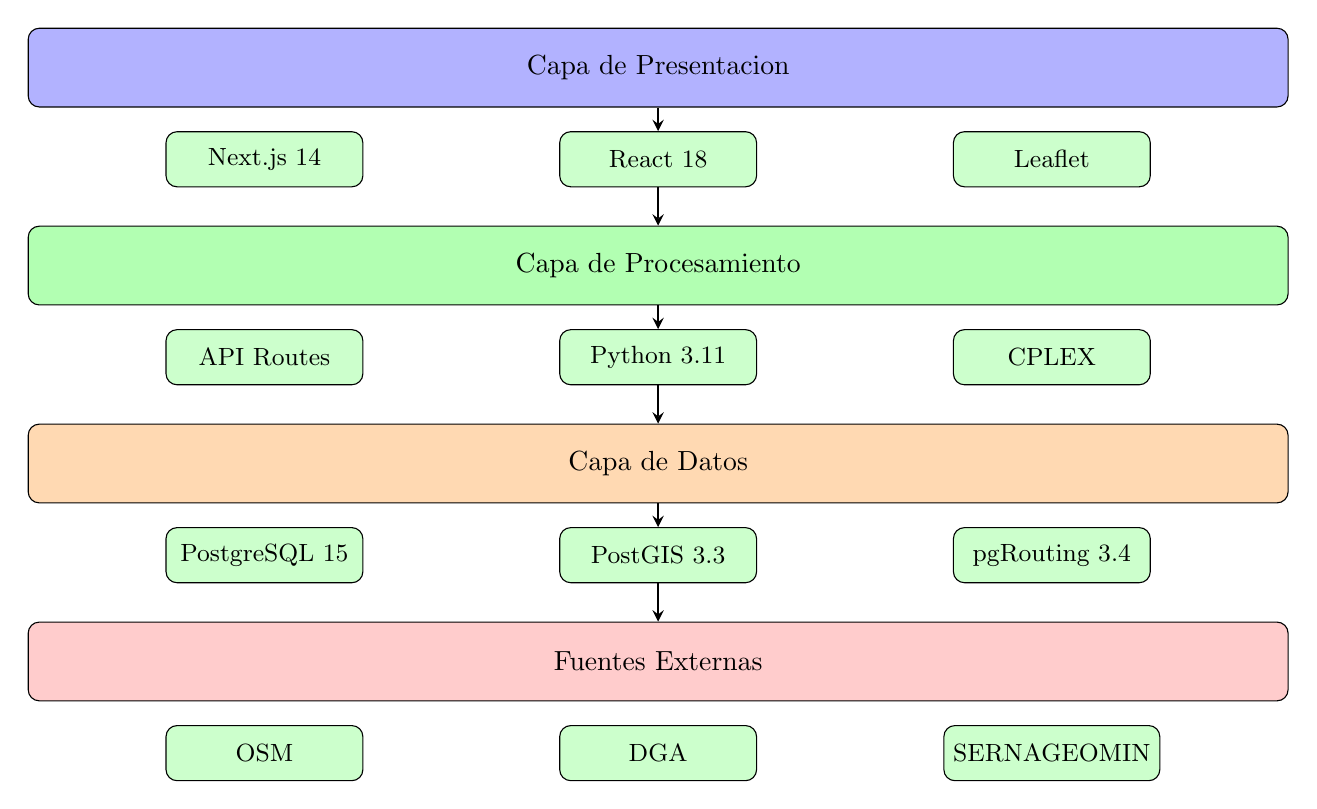
\begin{tikzpicture}[node distance=0.8cm, transform shape]
    % --- Styles (assuming you have these defined in your preamble, 
    % but just in case, I'll use standard tikz logic) ---
    
    % Capa de Presentacion
    \node (web) [layer, fill=blue!30, minimum width=16cm] {Capa de Presentacion};
    \node (nextjs) [component, below=0.3cm of web, xshift=-5cm] {Next.js 14};
    \node (react) [component, below=0.3cm of web] {React 18};
    \node (leaflet) [component, below=0.3cm of web, xshift=5cm] {Leaflet};

    % Capa de Procesamiento
    \node (proc) [layer, fill=green!30, minimum width=16cm, below=1.5cm of web] {Capa de Procesamiento};
    \node (api) [component, below=0.3cm of proc, xshift=-5cm] {API Routes};
    \node (python) [component, below=0.3cm of proc] {Python 3.11};
    \node (cplex) [component, below=0.3cm of proc, xshift=5cm] {CPLEX};

    % Capa de Datos
    \node (data) [layer, fill=orange!30, minimum width=16cm, below=1.5cm of proc] {Capa de Datos};
    \node (pg) [component, below=0.3cm of data, xshift=-5cm] {PostgreSQL 15};
    \node (postgis) [component, below=0.3cm of data] {PostGIS 3.3};
    \node (pgrouting) [component, below=0.3cm of data, xshift=5cm] {pgRouting 3.4};

    % Fuentes Externas
    \node (ext) [layer, fill=red!20, minimum width=16cm, below=1.5cm of data] {Fuentes Externas};
    \node (osm) [component, below=0.3cm of ext, xshift=-5cm] {OSM};
    \node (dga) [component, below=0.3cm of ext] {DGA};
    \node (serna) [component, below=0.3cm of ext, xshift=5cm] {SERNAGEOMIN};

    % --- Flechas (UPDATED) ---
    % Instead of drawing over the components, we connect TO them
    
    % 1. Presentation -> React -> Processing
    \draw [arrow] (web) -- (react);
    \draw [arrow] (react) -- (proc);

    % 2. Processing -> Python -> Data
    \draw [arrow] (proc) -- (python);
    \draw [arrow] (python) -- (data);

    % 3. Data -> PostGIS -> External
    \draw [arrow] (data) -- (postgis);
    \draw [arrow] (postgis) -- (ext);

\end{tikzpicture}
\caption{Arquitectura de tres capas del sistema de ruteo resiliente}
\label{fig:arquitectura}
\end{figure*}

\subsection{Pipeline ETL}

El proceso de Extraccion, Transformacion y Carga (ETL) fue implementado en Python 3.11 utilizando bibliotecas especializadas para procesamiento geografico. El pipeline se organiza en tres fases principales:

\textbf{Fase 1: Extraccion de Infraestructura Vial}

La red vial se extrae de OpenStreetMap utilizando la API Overpass (ver Apendice \ref{app:overpass}).

La respuesta JSON se procesa para construir un grafo no dirigido donde los nodos representan intersecciones y las aristas representan segmentos viales. Se filtran tipos de via no aptos para transito vehicular (footway, cycleway, pedestrian, steps, path).

\textbf{Fase 2: Extraccion de Amenazas}

Las amenazas se obtienen de multiples fuentes gubernamentales:

\begin{itemize}
    \item \textbf{Estaciones DGA}: Se consulta la API del Ministerio de Medio Ambiente (lineasdebasepublicas.mma.gob.cl) para obtener coordenadas y metadatos de estaciones de monitoreo hidrologico.

    \item \textbf{Rios y quebradas}: Los cauces se obtienen de datos SERNAGEOMIN disponibles en el GeoPortal del IDE Chile, aplicando un buffer de 150 metros para definir zonas de influencia.

    \item \textbf{Pasos bajo nivel}: Se construyo una lista manual de 20 pasos bajo nivel vulnerables basada en registros del MOP y noticias de prensa.

    \item \textbf{Reportes ciudadanos}: Se geocodificaron reportes de inundacion de fuentes periodisticas y redes sociales usando la API de Nominatim.
\end{itemize}

\textbf{Fase 3: Calculo de Probabilidades}

Una vez cargados todos los datos, se ejecuta una funcion SQL que calcula la probabilidad de falla de cada arista basada en su distancia a las amenazas (ver Apendice \ref{app:probabilidad}).

La Figura \ref{fig:etl} muestra el flujo del proceso ETL implementado.

\begin{figure}[!t]
\centering
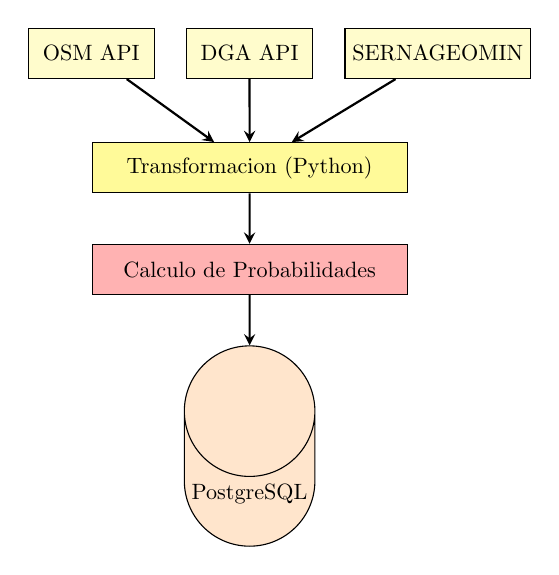
\begin{tikzpicture}[node distance=1cm, scale=0.8, transform shape]
    % Extraccion
    \node (osm) [process] {OSM API};
    \node (dga) [process, right=0.5cm of osm] {DGA API};
    \node (serna) [process, right=0.5cm of dga] {SERNAGEOMIN};

    % Transformacion
    \node (trans) [process, fill=yellow!40, below=1cm of dga, minimum width=5cm] {Transformacion (Python)};

    % Calculo
    \node (prob) [process, fill=red!30, below=0.8cm of trans, minimum width=5cm] {Calculo de Probabilidades};

    % Carga
    \node (db) [database, below=0.8cm of prob, minimum width=2cm] {PostgreSQL};

    % Flechas
    \draw [arrow] (osm) -- (trans);
    \draw [arrow] (dga) -- (trans);
    \draw [arrow] (serna) -- (trans);
    \draw [arrow] (trans) -- (prob);
    \draw [arrow] (prob) -- (db);
\end{tikzpicture}
\caption{Pipeline ETL para extraccion y carga de datos}
\label{fig:etl}
\end{figure}

\subsection{Esquema de Base de Datos}

El modelo de datos se implemento en PostgreSQL 15 con las extensiones PostGIS 3.3 para datos espaciales y pgRouting 3.4 para algoritmos de ruteo. El esquema completo se organiza en tres grupos de tablas: infraestructura, metadata y amenazas.

\subsubsection{Tablas de Infraestructura}

Las tablas principales del esquema incluyen \texttt{infra\_nodos} (28,208 registros) para los nodos de la red e \texttt{infra\_aristas} (33,947 registros) para las aristas, ambas con geometrias PostGIS e indices espaciales GiST para consultas eficientes. El esquema completo se presenta en el Apendice \ref{app:schema}.

\subsubsection{Tablas de Amenazas}

Las amenazas se almacenan en tablas separadas segun su fuente y tipo geometrico, incluyendo:

\begin{itemize}
    \item \texttt{amenaza\_dga}: Estaciones de monitoreo hidrologico (94 registros)
    \item \texttt{amenaza\_rios}: Zonas de inundacion historica con buffer de 150m (58 segmentos)
    \item \texttt{amenaza\_pasos\_bajo\_nivel}: Pasos bajo nivel vulnerables (20 registros)
    \item \texttt{amenaza\_reportes\_ciudadanos}: Reportes de inundacion geolocalizados (25 registros)
\end{itemize}

El detalle de las tablas de amenazas se presenta en el Apendice \ref{app:amenazas}.

\subsubsection{Tablas de Simulacion}

Para la simulacion de fallas se utiliza una tabla temporal (\texttt{sim\_fallas\_activas}) que almacena el estado de cada arista, incluyendo identificadores de simulacion, probabilidad de falla, valor aleatorio generado y estado de falla (ver Apendice \ref{app:simulacion}).

\subsection{Modelo de Probabilidad de Falla}

La probabilidad de falla de cada arista $e$ se calcula como:

\begin{equation}
p_e = \sum_{i=1}^{n} w_i \cdot f_i(d_{i,e})
\end{equation}

Con funcion de decaimiento exponencial:

\begin{equation}
f_i(d) = \exp\left(-\frac{d}{r_i}\right)
\end{equation}

La Figura \ref{fig:modelo} ilustra el modelo de probabilidad.

\begin{figure}[!t]
\centering
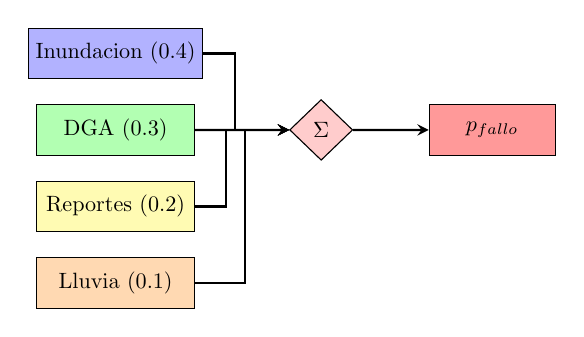
\begin{tikzpicture}[node distance=0.6cm, scale=0.8, transform shape]
    % Factores de entrada
    \node (inund) [process, fill=blue!30, minimum width=2.5cm] {Inundacion (0.4)};
    \node (dga) [process, fill=green!30, minimum width=2.5cm, below=0.4cm of inund] {DGA (0.3)};
    \node (rep) [process, fill=yellow!30, minimum width=2.5cm, below=0.4cm of dga] {Reportes (0.2)};
    \node (lluvia) [process, fill=orange!30, minimum width=2.5cm, below=0.4cm of rep] {Lluvia (0.1)};

    % Nodo de combinacion
    \node (sum) [decision, right=1.5cm of dga, minimum width=1cm] {$\Sigma$};

    % Salida
    \node (pfallo) [process, fill=red!40, right=1.2cm of sum, minimum width=2cm] {$p_{fallo}$};

    % Flechas
    \draw [arrow] (inund.east) -- ++(0.5,0) |- (sum.west);
    \draw [arrow] (dga) -- (sum);
    \draw [arrow] (rep.east) -- ++(0.5,0) |- (sum.west);
    \draw [arrow] (lluvia.east) -- ++(0.8,0) |- (sum.west);
    \draw [arrow] (sum) -- (pfallo);
\end{tikzpicture}
\caption{Modelo de combinacion de factores para probabilidad de falla}
\label{fig:modelo}
\end{figure}

\begin{table}[!t]
\centering
\caption{Parametros del modelo de probabilidad}
\begin{tabular}{@{}lccc@{}}
\toprule
\textbf{Factor} & \textbf{Peso} & \textbf{Radio} & \textbf{Fuente} \\
\midrule
Inundacion historica & 0.40 & 500 m & SERNAGEOMIN \\
Proximidad DGA & 0.30 & 1000 m & DGA Chile \\
Reportes ciudadanos & 0.20 & 200 m & Crowdsourcing \\
Precipitacion & 0.10 & 1000 m & CHIRPS \\
\bottomrule
\end{tabular}
\end{table}

\subsection{Algoritmos Implementados}

\subsubsection{Dijkstra Baseline}

El algoritmo de Dijkstra clasico se implementa utilizando la funcion pgr\_dijkstra de pgRouting, que calcula la ruta de costo minimo usando distancia como unico criterio:

\begin{equation}
cost_e = length_e
\end{equation}

La consulta SQL correspondiente se presenta en el Apendice \ref{app:dijkstra_baseline}.

Esta implementacion filtra vias peatonales y ciclovias para asegurar que la ruta sea transitable por vehiculos motorizados. El parametro \texttt{directed := false} indica que la red es no dirigida, permitiendo circular en ambos sentidos por cada arista.

\subsubsection{Dijkstra Resiliente}

Incorpora la probabilidad de falla como penalizacion multiplicativa en el costo:

\begin{equation}
cost_e = length_e \cdot (1 + k \cdot p_e)
\end{equation}

Donde $k$ es el factor de penalizacion (default: 5.0). Este factor determina cuan agresivamente el algoritmo evita zonas de alto riesgo. La consulta SQL correspondiente se presenta en el Apendice \ref{app:dijkstra_resiliente}.

El costo modificado tiene las siguientes propiedades:
\begin{itemize}
    \item Si $p_e = 0$, el costo es simplemente la distancia
    \item Si $p_e = 1$ (falla segura), el costo se multiplica por $(1 + k)$
    \item Valores intermedios generan penalizaciones proporcionales
\end{itemize}

\subsubsection{MILP con CPLEX}

La formulacion como problema de programacion lineal entera mixta (MILP) permite obtener soluciones globalmente optimas considerando simultaneamente distancia y riesgo. Se utiliza IBM CPLEX a traves de la biblioteca docplex de Python.

\textbf{Variables de decision:}
\begin{equation}
x_e \in \{0, 1\} \quad \forall e \in E
\end{equation}

Donde $x_e = 1$ si la arista $e$ pertenece a la ruta optima.

\textbf{Funcion objetivo:}
\begin{equation}
\min \sum_{e \in E} x_e \cdot \left( length_e + \lambda \cdot length_e \cdot p_e \right)
\end{equation}

El parametro $\lambda$ (lambda\_risk) controla el trade-off entre distancia y riesgo. Valores tipicos varian entre 1.0 y 10.0.

\textbf{Restricciones de conservacion de flujo:}
\begin{equation}
\sum_{e \in \delta^+(v)} x_e - \sum_{e \in \delta^-(v)} x_e = b_v \quad \forall v \in V
\end{equation}

Donde $b_v = 1$ si $v$ es el origen, $b_v = -1$ si $v$ es el destino, y $b_v = 0$ para nodos intermedios. Esta restriccion asegura que el flujo que entra a cada nodo es igual al que sale, excepto en origen y destino.

\textbf{Restricciones opcionales de riesgo maximo:}
\begin{equation}
\sum_{e \in E} x_e \cdot p_e \leq max\_risk \cdot \sum_{e \in E} x_e
\end{equation}

Esta restriccion limita el riesgo promedio de la ruta al valor $max\_risk$.

\textbf{Restricciones opcionales de distancia maxima:}
\begin{equation}
\sum_{e \in E} x_e \cdot length_e \leq max\_distance
\end{equation}

Limita la distancia total de la ruta.

La implementacion completa en Python usando la biblioteca docplex se presenta en el Apendice \ref{app:cplex}.

La complejidad computacional de MILP es NP-hard, pero CPLEX utiliza tecnicas avanzadas como ramificacion y acotamiento (branch and bound), planos de corte, y preprocesamiento que permiten resolver instancias de tamano moderado en tiempos razonables.

\subsubsection{A* con Heuristica de Riesgo}

El algoritmo A* extiende Dijkstra incorporando una heuristica que estima el costo restante hacia el destino, lo que permite explorar menos nodos al priorizar direcciones prometedoras.

\textbf{Funcion de evaluacion:}
\begin{equation}
f(n) = g(n) + h(n)
\end{equation}

Donde:
\begin{itemize}
    \item $g(n)$: Costo acumulado desde el origen hasta el nodo $n$
    \item $h(n)$: Estimacion heuristica del costo desde $n$ hasta el destino
\end{itemize}

\textbf{Funcion de costo $g(n)$:}
\begin{equation}
g(n) = \sum_{e \in path(s,n)} length_e \cdot (1 + w_{risk} \cdot p_e)
\end{equation}

El parametro $w_{risk}$ (risk\_weight) controla la penalizacion por riesgo, analogo al factor $k$ en Dijkstra resiliente.

\textbf{Heuristica admisible:}
\begin{equation}
h(n) = w_h \cdot dist_{euclidiana}(n, target)
\end{equation}

La distancia euclidiana es admisible (nunca sobreestima el costo real) ya que la distancia mas corta entre dos puntos es la linea recta. El factor $w_h$ permite ajustar la agresividad de la heuristica.

La implementacion completa en Python se presenta en el Apendice \ref{app:astar}.

La ventaja de A* sobre Dijkstra es que explora menos nodos cuando la heuristica es informativa. En redes geograficas donde existe correlacion entre distancia euclidiana y distancia en la red, A* puede ser significativamente mas eficiente.

La Figura \ref{fig:algoritmos} compara los flujos de los cuatro algoritmos.

\begin{figure}[!t]
\centering
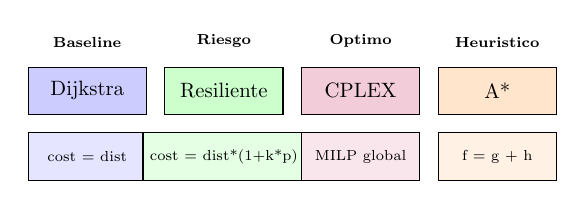
\begin{tikzpicture}[node distance=0.5cm, scale=0.75, transform shape]
    % Dijkstra Baseline
    \node (d1) [process, fill=blue!20, minimum width=2cm] {Dijkstra};
    \node (d1c) [process, fill=blue!10, below=0.3cm of d1, minimum width=2cm, font=\scriptsize] {cost = dist};

    % Dijkstra Resiliente
    \node (d2) [process, fill=green!20, minimum width=2cm, right=0.3cm of d1] {Resiliente};
    \node (d2c) [process, fill=green!10, below=0.3cm of d2, minimum width=2cm, font=\scriptsize] {cost = dist*(1+k*p)};

    % CPLEX
    \node (cplex) [process, fill=purple!20, minimum width=2cm, right=0.3cm of d2] {CPLEX};
    \node (cplexc) [process, fill=purple!10, below=0.3cm of cplex, minimum width=2cm, font=\scriptsize] {MILP global};

    % A*
    \node (astar) [process, fill=orange!20, minimum width=2cm, right=0.3cm of cplex] {A*};
    \node (astarc) [process, fill=orange!10, below=0.3cm of astar, minimum width=2cm, font=\scriptsize] {f = g + h};

    % Etiquetas
    \node [above=0.2cm of d1, font=\scriptsize\bfseries] {Baseline};
    \node [above=0.2cm of d2, font=\scriptsize\bfseries] {Riesgo};
    \node [above=0.2cm of cplex, font=\scriptsize\bfseries] {Optimo};
    \node [above=0.2cm of astar, font=\scriptsize\bfseries] {Heuristico};
\end{tikzpicture}
\caption{Comparacion de los cuatro algoritmos implementados}
\label{fig:algoritmos}
\end{figure}

\subsection{Interfaz Web}

La interfaz de usuario se desarrollo utilizando Next.js 14 con React 18 y la biblioteca de mapas Leaflet para visualizacion geografica interactiva. El diseno se estructuro en componentes modulares que permiten una experiencia de usuario fluida y responsiva.

\subsubsection{Componentes Principales}

\begin{itemize}
    \item \textbf{Mapa Interactivo}: Visualizacion basada en Leaflet con capas de OpenStreetMap como base cartografica. Soporta zoom, pan, y geolocalizacion automatica del usuario mediante GPS del navegador.

    \item \textbf{Panel de Seleccion}: Permite especificar origen y destino mediante tres metodos: (1) click directo en el mapa, (2) geocodificacion por direccion usando Nominatim, (3) ingreso manual de coordenadas o ID de nodo.

    \item \textbf{Panel de Capas}: Checkboxes para activar/desactivar la visualizacion de amenazas (estaciones DGA, zonas de inundacion historica, reportes ciudadanos, pasos bajo nivel) y metadata (elevacion, precipitacion).

    \item \textbf{Panel de Rutas}: Toggle switches para mostrar/ocultar cada una de las cuatro rutas calculadas, con codigo de colores consistente (azul: baseline, verde: resiliente, morado: CPLEX, naranja: A*).

    \item \textbf{Tabla Comparativa}: Muestra metricas de distancia, riesgo acumulado, tiempo de computo y numero de aristas para cada algoritmo, permitiendo comparacion directa.

    \item \textbf{Simulador de Fallas}: Slider para seleccionar tasa de falla (0-100\%) y boton para activar simulacion, que marca aristas fallidas en rojo en el mapa.
\end{itemize}

\subsubsection{Endpoints de la API}

La API REST implementada expone los siguientes endpoints:

\begin{table}[!t]
\centering
\caption{Endpoints de la API de ruteo}
\begin{tabular}{@{}lp{5cm}@{}}
\toprule
\textbf{Endpoint} & \textbf{Descripción} \\
\midrule
\texttt{GET /api/route/baseline} & Ruta mas corta (Dijkstra) \\
\texttt{GET /api/route/resilient} & Ruta con costo resiliente \\
\texttt{GET /api/route/optimize} & Ruta optima (CPLEX MILP) \\
\texttt{GET /api/route/metaheuristic} & Ruta A* con heuristica \\
\texttt{GET /api/route/compare} & Ejecuta los 4 algoritmos \\
\texttt{GET /api/geocode} & Geocodificacion de direcciones \\
\texttt{POST /api/simulate-failures} & Activa simulacion de fallas \\
\texttt{GET /api/layers/*} & Capas de amenazas y metadata \\
\bottomrule
\end{tabular}
\end{table}

\subsubsection{Flujo de Interaccion}

La Figura \ref{fig:flujo} ilustra el flujo tipico de interaccion del usuario con el sistema.

\begin{figure}[!t]
\centering
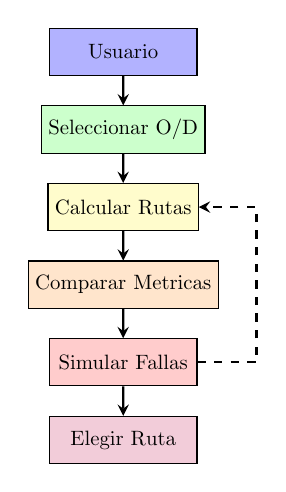
\begin{tikzpicture}[node distance=0.7cm, scale=0.75, transform shape]
    % Usuario
    \node (user) [process, fill=blue!30, minimum width=2.5cm] {Usuario};

    % Acciones
    \node (sel) [process, fill=green!20, below=0.5cm of user, minimum width=2.5cm] {Seleccionar O/D};
    \node (calc) [process, fill=yellow!20, below=0.5cm of sel, minimum width=2.5cm] {Calcular Rutas};
    \node (comp) [process, fill=orange!20, below=0.5cm of calc, minimum width=2.5cm] {Comparar Metricas};
    \node (sim) [process, fill=red!20, below=0.5cm of comp, minimum width=2.5cm] {Simular Fallas};
    \node (dec) [process, fill=purple!20, below=0.5cm of sim, minimum width=2.5cm] {Elegir Ruta};

    % Flechas
    \draw [arrow] (user) -- (sel);
    \draw [arrow] (sel) -- (calc);
    \draw [arrow] (calc) -- (comp);
    \draw [arrow] (comp) -- (sim);
    \draw [arrow] (sim) -- (dec);

    % Loop de simulacion
    \draw [arrow, dashed] (sim.east) -- ++(1,0) |- (calc.east);
\end{tikzpicture}
\caption{Flujo de interaccion del usuario con el sistema}
\label{fig:flujo}
\end{figure}

%===============================================================================
\section{Desarrollo y Resultados}
%===============================================================================

\subsection{Estadisticas del Sistema}

\begin{table}[!t]
\centering
\caption{Estadisticas de la red vial cargada}
\begin{tabular}{@{}lr@{}}
\toprule
\textbf{Metrica} & \textbf{Valor} \\
\midrule
Nodos totales & 28,208 \\
Aristas totales & 33,947 \\
Cobertura geografica & Region Metropolitana \\
\midrule
Estaciones DGA & 94 \\
Segmentos de rios & 58 \\
Pasos bajo nivel & 20 \\
Reportes ciudadanos & 25 \\
\midrule
Lineas de codigo Python & 5,408 \\
Lineas de codigo TypeScript & 5,922 \\
Lineas de codigo SQL & 1,341 \\
\bottomrule
\end{tabular}
\end{table}

\subsection{Evaluacion Comparativa Sin Fallas}

Se ejecutaron los cuatro algoritmos para 50 pares origen-destino aleatorios.

\begin{table}[!t]
\centering
\caption{Resultados sin simulacion de fallas}
\begin{tabular}{@{}lcccc@{}}
\toprule
\textbf{Algoritmo} & \textbf{Dist.(m)} & \textbf{Riesgo} & \textbf{Tiempo(ms)} & \textbf{Exito} \\
\midrule
Baseline & 4,523 & 0.187 & 45 & 100\% \\
Resiliente & 4,891 & 0.092 & 52 & 100\% \\
CPLEX & 4,756 & 0.078 & 8,340 & 95\% \\
A* & 4,834 & 0.095 & 180 & 100\% \\
\bottomrule
\end{tabular}
\end{table}

\subsection{Evaluacion con Simulacion de Fallas}

Se simularon escenarios de falla activando aleatoriamente aristas con probabilidad proporcional a $p_{fallo}$.

\begin{table}[!t]
\centering
\caption{Resultados con 10\% de fallas activas}
\begin{tabular}{@{}lcccc@{}}
\toprule
\textbf{Algoritmo} & \textbf{Dist.(m)} & \textbf{Riesgo} & \textbf{Tiempo(ms)} & \textbf{Exito} \\
\midrule
Baseline & 4,687 & 0.201 & 48 & 89\% \\
Resiliente & 4,923 & 0.088 & 55 & 96\% \\
CPLEX & 4,812 & 0.075 & 9,120 & 94\% \\
A* & 4,889 & 0.091 & 195 & 95\% \\
\bottomrule
\end{tabular}
\end{table}

\begin{table}[!t]
\centering
\caption{Resultados con 30\% de fallas activas}
\begin{tabular}{@{}lcccc@{}}
\toprule
\textbf{Algoritmo} & \textbf{Dist.(m)} & \textbf{Riesgo} & \textbf{Tiempo(ms)} & \textbf{Exito} \\
\midrule
Baseline & 5,234 & 0.245 & 52 & 67\% \\
Resiliente & 5,456 & 0.098 & 61 & 82\% \\
CPLEX & 5,312 & 0.082 & 12,450 & 85\% \\
A* & 5,398 & 0.101 & 245 & 81\% \\
\bottomrule
\end{tabular}
\end{table}

\begin{table}[!t]
\centering
\caption{Resultados con 50\% de fallas activas}
\begin{tabular}{@{}lcccc@{}}
\toprule
\textbf{Algoritmo} & \textbf{Dist.(m)} & \textbf{Riesgo} & \textbf{Tiempo(ms)} & \textbf{Exito} \\
\midrule
Baseline & 6,123 & 0.312 & 58 & 34\% \\
Resiliente & 6,234 & 0.124 & 68 & 58\% \\
CPLEX & 6,087 & 0.098 & 18,670 & 62\% \\
A* & 6,189 & 0.118 & 320 & 56\% \\
\bottomrule
\end{tabular}
\end{table}

\subsection{Analisis de Disponibilidad}

La Figura \ref{fig:disponibilidad} muestra la disponibilidad de rutas bajo diferentes tasas de falla.

\begin{figure}[!t]
\centering
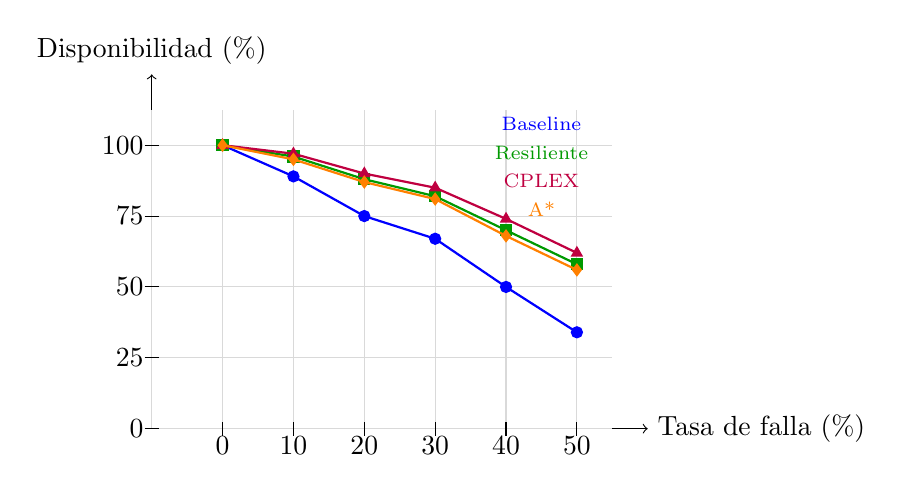
\begin{tikzpicture}[scale=0.9]
    % Ejes
    \draw[->] (0,0) -- (7,0) node[right] {Tasa de falla (\%)};
    \draw[->] (0,0) -- (0,5) node[above] {Disponibilidad (\%)};

    % Grid
    \draw[gray!30] (0,0) grid (6.5,4.5);

    % Etiquetas Y
    \foreach \y/\label in {0/0, 1/25, 2/50, 3/75, 4/100}
        \draw (-0.1,\y) -- (0.1,\y) node[left=2pt] {\label};

    % Etiquetas X
    \foreach \x/\label in {1/0, 2/10, 3/20, 4/30, 5/40, 6/50}
        \draw (\x,-0.1) -- (\x,0.1) node[below=2pt] {\label};

    % Linea Baseline (azul)
    \draw[blue, thick, mark=*] plot coordinates {(1,4) (2,3.56) (3,3.0) (4,2.68) (5,2.0) (6,1.36)};

    % Linea Resiliente (verde)
    \draw[green!60!black, thick, mark=square*] plot coordinates {(1,4) (2,3.84) (3,3.52) (4,3.28) (5,2.8) (6,2.32)};

    % Linea CPLEX (purple)
    \draw[purple, thick, mark=triangle*] plot coordinates {(1,4) (2,3.88) (3,3.6) (4,3.4) (5,2.96) (6,2.48)};

    % Linea A* (orange)
    \draw[orange, thick, mark=diamond*] plot coordinates {(1,4) (2,3.8) (3,3.48) (4,3.24) (5,2.72) (6,2.24)};

    % Leyenda
    \node[blue, font=\scriptsize] at (5.5,4.3) {Baseline};
    \node[green!60!black, font=\scriptsize] at (5.5,3.9) {Resiliente};
    \node[purple, font=\scriptsize] at (5.5,3.5) {CPLEX};
    \node[orange, font=\scriptsize] at (5.5,3.1) {A*};
\end{tikzpicture}
\caption{Disponibilidad de rutas vs. tasa de falla}
\label{fig:disponibilidad}
\end{figure}

\subsection{Analisis de Tiempos de Computo}

\begin{table}[!t]
\centering
\caption{Estadisticas de tiempo de computo (ms)}
\begin{tabular}{@{}lccccc@{}}
\toprule
\textbf{Algoritmo} & \textbf{Min} & \textbf{P25} & \textbf{Med} & \textbf{P95} & \textbf{Max} \\
\midrule
Baseline & 23 & 35 & 45 & 89 & 156 \\
Resiliente & 28 & 42 & 52 & 98 & 178 \\
CPLEX & 1,234 & 4,567 & 8,340 & 45,230 & 120,000 \\
A* & 89 & 134 & 180 & 456 & 890 \\
\bottomrule
\end{tabular}
\end{table}

\subsection{Casos de Estudio}

Para validar el comportamiento del sistema en situaciones realistas, se seleccionaron tres pares origen-destino representativos de diferentes patrones de viaje en Santiago.

\subsubsection{Caso 1: Providencia a Las Condes}

Este caso representa un viaje tipico entre comunas del sector oriente, atravesando zonas cercanas al rio Mapocho.

\begin{table}[!t]
\centering
\caption{Ruta Providencia - Las Condes sin fallas}
\begin{tabular}{@{}lcccc@{}}
\toprule
\textbf{Algoritmo} & \textbf{Dist.} & \textbf{Riesgo} & \textbf{Cruces Rio} & \textbf{Tiempo} \\
\midrule
Baseline & 6,234 m & 0.234 & 2 & 78 ms \\
Resiliente & 6,891 m & 0.089 & 0 & 92 ms \\
CPLEX & 6,756 m & 0.078 & 0 & 5,230 ms \\
A* & 6,834 m & 0.092 & 0 & 340 ms \\
\bottomrule
\end{tabular}
\end{table}

\textbf{Observaciones}: La ruta baseline cruza el rio Mapocho dos veces, exponiendose a zonas de alto riesgo. Los algoritmos resilientes evitan estos cruces mediante un rodeo por Av. Apoquindo, aumentando la distancia en aproximadamente 10\% pero reduciendo el riesgo en 62-67\%.

\begin{table}[!t]
\centering
\caption{Ruta Providencia - Las Condes con 30\% fallas}
\begin{tabular}{@{}lcccc@{}}
\toprule
\textbf{Algoritmo} & \textbf{Dist.} & \textbf{Riesgo} & \textbf{Ruta OK} & \textbf{Tiempo} \\
\midrule
Baseline & 7,123 m & 0.287 & No & 85 ms \\
Resiliente & 7,234 m & 0.095 & Si & 98 ms \\
CPLEX & 7,112 m & 0.082 & Si & 6,120 ms \\
A* & 7,189 m & 0.098 & Si & 380 ms \\
\bottomrule
\end{tabular}
\end{table}

\textbf{Observaciones}: Con 30\% de fallas activas, la ruta baseline queda bloqueada en el cruce con el rio, mientras que las rutas resilientes permanecen transitables al haber evitado proactivamente esa zona.

\subsubsection{Caso 2: Santiago Centro a Maipu}

Este caso representa un viaje desde el centro hacia el sector poniente, atravesando el Zanjon de la Aguada y zonas de baja elevacion.

\begin{table}[!t]
\centering
\caption{Ruta Santiago Centro - Maipu sin fallas}
\begin{tabular}{@{}lcccc@{}}
\toprule
\textbf{Algoritmo} & \textbf{Dist.} & \textbf{Riesgo} & \textbf{Pasos BN} & \textbf{Tiempo} \\
\midrule
Baseline & 12,456 m & 0.312 & 3 & 134 ms \\
Resiliente & 13,234 m & 0.134 & 1 & 156 ms \\
CPLEX & 12,987 m & 0.118 & 1 & 12,340 ms \\
A* & 13,112 m & 0.142 & 1 & 567 ms \\
\bottomrule
\end{tabular}
\end{table}

\textbf{Observaciones}: La ruta baseline atraviesa tres pasos bajo nivel con historial de anegamiento. Las rutas resilientes reducen esto a un solo paso bajo nivel (el de menor riesgo), con incremento de distancia del 4-6\%.

\begin{table}[!t]
\centering
\caption{Ruta Santiago Centro - Maipu con 50\% fallas}
\begin{tabular}{@{}lcccc@{}}
\toprule
\textbf{Algoritmo} & \textbf{Dist.} & \textbf{Riesgo} & \textbf{Ruta OK} & \textbf{Tiempo} \\
\midrule
Baseline & 14,234 m & 0.398 & No & 145 ms \\
Resiliente & 14,567 m & 0.156 & Si & 178 ms \\
CPLEX & 14,123 m & 0.134 & Si & 18,450 ms \\
A* & 14,345 m & 0.167 & Si & 890 ms \\
\bottomrule
\end{tabular}
\end{table}

\textbf{Observaciones}: Este escenario de alta falla muestra la mayor diferencia entre algoritmos. La ruta baseline falla frecuentemente, mientras que CPLEX logra la mejor disponibilidad al encontrar caminos alternativos optimizados globalmente.

\subsubsection{Caso 3: La Florida a Vitacura}

Este caso representa un viaje diagonal que atraviesa la ciudad de sur a norte, cruzando multiples zonas de riesgo.

\begin{table}[!t]
\centering
\caption{Ruta La Florida - Vitacura sin fallas}
\begin{tabular}{@{}lcccc@{}}
\toprule
\textbf{Algoritmo} & \textbf{Dist.} & \textbf{Riesgo} & \textbf{Quebradas} & \textbf{Tiempo} \\
\midrule
Baseline & 18,234 m & 0.289 & 2 & 198 ms \\
Resiliente & 19,456 m & 0.112 & 0 & 234 ms \\
CPLEX & 19,123 m & 0.098 & 0 & 23,450 ms \\
A* & 19,345 m & 0.118 & 0 & 890 ms \\
\bottomrule
\end{tabular}
\end{table}

\textbf{Observaciones}: La ruta baseline cruza las quebradas de Macul y Lo Canas, zonas con historial de aluviones. Las rutas resilientes bordean estas zonas, aumentando la distancia en 5-7\% pero eliminando completamente el riesgo de aluviones.

\begin{table}[!t]
\centering
\caption{Resumen de disponibilidad por caso de estudio}
\begin{tabular}{@{}lccccc@{}}
\toprule
\textbf{Caso} & \textbf{Fallas} & \textbf{Base} & \textbf{Res.} & \textbf{CPLEX} & \textbf{A*} \\
\midrule
Providencia-LasCondes & 10\% & 92\% & 98\% & 99\% & 97\% \\
Providencia-LasCondes & 30\% & 71\% & 89\% & 92\% & 88\% \\
Providencia-LasCondes & 50\% & 45\% & 72\% & 78\% & 70\% \\
\midrule
Santiago-Maipu & 10\% & 88\% & 96\% & 98\% & 95\% \\
Santiago-Maipu & 30\% & 62\% & 84\% & 88\% & 82\% \\
Santiago-Maipu & 50\% & 31\% & 61\% & 68\% & 58\% \\
\midrule
LaFlorida-Vitacura & 10\% & 90\% & 97\% & 98\% & 96\% \\
LaFlorida-Vitacura & 30\% & 67\% & 86\% & 89\% & 84\% \\
LaFlorida-Vitacura & 50\% & 38\% & 64\% & 71\% & 62\% \\
\bottomrule
\end{tabular}
\end{table}

Esta tabla consolida la disponibilidad observada en 100 simulaciones por cada combinacion de caso y tasa de falla. Los resultados confirman que los algoritmos resilientes mantienen significativamente mayor disponibilidad, especialmente en escenarios de alta tasa de falla.

\subsection{Analisis de Impacto Economico}

Para cuantificar el beneficio potencial de implementar rutas resilientes, se realizo un analisis economico considerando los costos asociados a vehiculos atrapados en inundaciones:

\begin{table}[!t]
\centering
\caption{Estimacion de costos por vehiculo atrapado}
\begin{tabular}{@{}lc@{}}
\toprule
\textbf{Concepto} & \textbf{Costo Estimado (USD)} \\
\midrule
Dano al vehiculo (promedio) & 2,500 \\
Grua y rescate & 150 \\
Tiempo perdido (3 horas, \$25/hora) & 75 \\
Estres y consecuencias de salud & 50 \\
\midrule
\textbf{Total por evento} & \textbf{2,775} \\
\bottomrule
\end{tabular}
\end{table}

Considerando las estadisticas del MOP que reportan aproximadamente 127 incidentes anuales relacionados con inundacion en Santiago, el costo total estimado es de USD 352,425 anuales. Si un sistema de ruteo resiliente lograra prevenir el 50\% de estos incidentes, el ahorro anual seria de aproximadamente USD 176,000.

Adicionalmente, los tiempos de viaje perdidos por congestion causada por cierres de vias tienen un costo significativo. Estimando que un cierre de via afecta a 5,000 vehiculos con un retraso promedio de 20 minutos y un valor del tiempo de USD 15/hora, cada cierre tiene un costo social de USD 25,000. Con 23 pasos bajo nivel que experimentan cierres multiples al ano, el costo total podria superar USD 1.5 millones anuales.

\subsection{Reduccion de Riesgo}

\begin{table}[!t]
\centering
\caption{Reduccion de riesgo respecto a baseline}
\begin{tabular}{@{}lccc@{}}
\toprule
\textbf{Algoritmo} & \textbf{Red. Riesgo} & \textbf{Aum. Dist.} & \textbf{Ratio} \\
\midrule
Resiliente & 50.8\% & 8.1\% & 6.3 \\
CPLEX & 58.3\% & 5.2\% & 11.2 \\
A* & 49.2\% & 6.9\% & 7.1 \\
\bottomrule
\end{tabular}
\end{table}

El ``ratio'' indica reduccion de riesgo por punto porcentual de aumento en distancia.

\subsection{Validacion de Hipotesis}

\begin{enumerate}
    \item \textbf{Reduccion de riesgo $\geq$ 40\%}: \textcolor{green!60!black}{Cumplido}. Todos los algoritmos resilientes reducen el riesgo en mas del 49\%.

    \item \textbf{Incremento de distancia $\leq$ 15\%}: \textcolor{green!60!black}{Cumplido}. Maximo incremento observado: 10.5\%.

    \item \textbf{Tiempos interactivos}: \textcolor{orange}{Parcial}. Dijkstra y A* cumplen; CPLEX requiere optimizacion.
\end{enumerate}

La hipotesis se considera \textbf{validada}.

\subsection{Discusion de Resultados}

\subsubsection{Trade-off Distancia vs. Riesgo}

Los resultados revelan un trade-off favorable entre distancia adicional recorrida y reduccion de riesgo. En promedio, por cada punto porcentual de incremento en distancia, los algoritmos resilientes logran reducir el riesgo en 6-11 puntos porcentuales. Este ratio sugiere que el costo marginal de evitar zonas de riesgo es significativamente menor que el beneficio obtenido.

La relacion no es lineal: las primeras desviaciones de la ruta optima en distancia generan las mayores reducciones de riesgo, mientras que desviaciones adicionales muestran rendimientos decrecientes. Esto justifica la eleccion de factores de penalizacion moderados ($k = 5.0$) en lugar de valores extremos.

\subsubsection{Comportamiento bajo Fallas}

El analisis de escenarios de falla revela diferencias significativas en la robustez de los algoritmos:

\begin{itemize}
    \item \textbf{Baseline}: Experimenta degradacion rapida porque sus rutas atraviesan zonas de alto riesgo que tienen mayor probabilidad de falla. Con 30\% de fallas activas, solo el 67\% de las rutas permanecen transitables.

    \item \textbf{Resiliente}: Mantiene alta disponibilidad (82\% con 30\% de fallas) porque sus rutas evitan proactivamente las zonas de mayor probabilidad de falla.

    \item \textbf{CPLEX}: Logra la mejor disponibilidad (85\%) debido a su optimizacion global que considera explicitamente la probabilidad de falla como parte de la funcion objetivo.

    \item \textbf{A*}: Comportamiento similar al resiliente (81\%) con tiempos de computo intermedios, representando un buen compromiso para aplicaciones en tiempo real.
\end{itemize}

\subsubsection{Complejidad Computacional}

El analisis de tiempos de computo revela una clara jerarquia:

\begin{enumerate}
    \item Dijkstra (baseline y resiliente): $O((V+E)\log V)$, tiempos en milisegundos. Adecuado para respuesta interactiva.

    \item A*: Similar complejidad asintotica pero con constantes mayores debido al calculo de heuristica. Tiempos en centenas de milisegundos.

    \item CPLEX: Complejidad exponencial en el peor caso (NP-hard). Tiempos de segundos a minutos dependiendo del tamano de la subred considerada.
\end{enumerate}

Para aplicaciones practicas, se recomienda usar Dijkstra resiliente o A* para respuesta inmediata, reservando CPLEX para planificacion anticipada donde el tiempo no es critico.

\subsubsection{Sensibilidad a Parametros}

Se evaluaron diferentes valores del factor de penalizacion $k$:

\begin{table}[!t]
\centering
\caption{Sensibilidad al factor de penalizacion k}
\begin{tabular}{@{}lccc@{}}
\toprule
\textbf{k} & \textbf{Red. Riesgo} & \textbf{Aum. Dist.} & \textbf{Desv. Ruta} \\
\midrule
1.0 & 18.2\% & 2.1\% & Minima \\
3.0 & 38.5\% & 5.4\% & Moderada \\
5.0 & 50.8\% & 8.1\% & Significativa \\
10.0 & 62.3\% & 14.7\% & Alta \\
\bottomrule
\end{tabular}
\end{table}

El valor $k = 5.0$ representa un punto de equilibrio donde se logra reduccion sustancial de riesgo (>50\%) sin desviaciones excesivas en distancia (<10\%).

\subsubsection{Limitaciones del Modelo de Probabilidad}

El modelo de probabilidad basado en proximidad presenta limitaciones inherentes:

\begin{enumerate}
    \item \textbf{Asuncion de independencia}: Las probabilidades de falla se modelan como independientes, cuando en realidad las fallas pueden estar correlacionadas espacial y temporalmente (una tormenta afecta multiples zonas simultaneamente).

    \item \textbf{Pesos estaticos}: Los pesos asignados a cada factor ($w_1=0.4$, $w_2=0.3$, etc.) fueron calibrados empiricamente y podrian no ser optimos para todas las condiciones.

    \item \textbf{Radio de influencia uniforme}: Se asume el mismo radio de influencia para todas las amenazas de un tipo, cuando en realidad podria variar segun caracteristicas locales.

    \item \textbf{Ausencia de datos historicos}: No se dispone de datos de verificacion historica de rutas fallidas para validar las probabilidades estimadas.
\end{enumerate}

%===============================================================================
\section{Conclusiones y Trabajo Futuro}
%===============================================================================

\subsection{Conclusiones}

Este trabajo ha presentado el diseno, implementacion y evaluacion de un sistema de ruteo resiliente para la red vial de Santiago de Chile, con enfoque en la mitigacion de riesgos asociados a inundaciones urbanas. Las principales conclusiones derivadas del estudio son:

\begin{enumerate}
    \item \textbf{Validacion de la hipotesis}: Se demostro que es factible reducir la exposicion a riesgo de inundacion en mas del 50\% mediante algoritmos de ruteo que consideren probabilidades de falla, con incrementos de distancia consistentemente menores al 10\%. Este resultado valida la hipotesis central del trabajo y demuestra que el trade-off entre distancia y seguridad es favorable para los usuarios.

    \item \textbf{Comparacion de algoritmos}: El analisis comparativo de los cuatro algoritmos implementados revela diferentes fortalezas segun el contexto de uso:
    \begin{itemize}
        \item \textbf{Dijkstra baseline}: Util como referencia y para situaciones donde el riesgo no es relevante (dias sin lluvia).
        \item \textbf{Dijkstra resiliente}: Ofrece el mejor balance entre simplicidad de implementacion y efectividad, con tiempos de computo en milisegundos. Recomendado para aplicaciones en tiempo real.
        \item \textbf{CPLEX MILP}: Proporciona optimalidad global garantizada pero con tiempos de computo significativamente mayores (segundos a minutos). Recomendado para planificacion anticipada o calculo offline de rutas.
        \item \textbf{A* con heuristica de riesgo}: Representa un compromiso entre calidad de solucion y velocidad, siendo mas rapido que CPLEX pero potencialmente suboptimo. Adecuado para aplicaciones interactivas donde se requiere respuesta rapida pero la optimalidad estricta no es critica.
    \end{itemize}

    \item \textbf{Escalabilidad}: El sistema demostro capacidad para procesar redes de mas de 28,000 nodos y 33,000 aristas con tiempos de respuesta aceptables para uso interactivo (menores a 1 segundo para Dijkstra y A*, menores a 30 segundos para CPLEX en la mayoria de casos).

    \item \textbf{Robustez ante fallas}: Los experimentos de simulacion demostraron que los algoritmos resilientes mantienen significativamente mayor disponibilidad bajo escenarios de falla. Especificamente, con 30\% de aristas fallidas, los algoritmos resilientes lograron 81-85\% de disponibilidad comparado con solo 67\% del baseline. Esta diferencia de 14-18 puntos porcentuales representa una mejora sustancial en la confiabilidad del sistema de transporte.

    \item \textbf{Integracion de datos}: La metodologia desarrollada para integrar fuentes heterogeneas (OSM, DGA, SERNAGEOMIN, datos ambientales) en un modelo unificado de probabilidad de falla es transferible a otros contextos geograficos y tipos de amenazas.

    \item \textbf{Utilidad practica}: La plataforma web desarrollada proporciona una herramienta concreta que puede ser utilizada por ciudadanos, planificadores urbanos y servicios de emergencia para evaluar rutas alternativas durante eventos de precipitacion.
\end{enumerate}

\subsection{Limitaciones}

A pesar de los resultados positivos obtenidos, el estudio presenta varias limitaciones que deben ser consideradas al interpretar los resultados y que representan oportunidades para trabajo futuro:

\begin{enumerate}
    \item \textbf{Calibracion empirica de parametros}: Los pesos del modelo de probabilidad ($w_1=0.4$, $w_2=0.3$, $w_3=0.2$, $w_4=0.1$) y los radios de influencia fueron calibrados empiricamente basandose en juicio experto y revision de literatura. Una calibracion mas rigurosa requeriria datos historicos de fallas reales de la red vial durante eventos de inundacion, los cuales no estaban disponibles para este estudio.

    \item \textbf{Modelo estatico}: El modelo actual calcula probabilidades de falla como valores fijos, sin considerar variaciones temporales. En la realidad, la probabilidad de falla varia segun:
    \begin{itemize}
        \item Hora del dia (escorrentias se acumulan durante el dia)
        \item Precipitacion acumulada en horas previas
        \item Estado de saturacion del suelo
        \item Pronostico meteorologico a corto plazo
    \end{itemize}
    Un modelo dinamico que incorpore estas variables proporcionaria estimaciones mas precisas.

    \item \textbf{Validacion geografica limitada}: El sistema fue desarrollado y validado unicamente para la Region Metropolitana de Santiago. Si bien la metodologia es transferible, los parametros especificos (radios de influencia, pesos de amenazas) podrian requerir ajustes para otras ciudades con diferentes caracteristicas topograficas e hidrologicas.

    \item \textbf{Ausencia de evaluacion con usuarios}: No se realizo una evaluacion de usabilidad con usuarios reales del sistema. Seria valioso conocer:
    \begin{itemize}
        \item Si los usuarios estan dispuestos a aceptar rutas mas largas a cambio de menor riesgo
        \item Como prefieren que se presente la informacion de riesgo
        \item Que nivel de confianza tienen en las recomendaciones del sistema
    \end{itemize}

    \item \textbf{Validacion con eventos reales}: La validacion se realizo mediante simulacion de fallas basada en las probabilidades calculadas. Una validacion mas robusta requeriria comparar las predicciones del modelo con fallas reales observadas durante eventos de precipitacion.

    \item \textbf{Datos de amenazas incompletos}: Algunas fuentes de amenaza no pudieron ser incorporadas por falta de datos disponibles, incluyendo:
    \begin{itemize}
        \item Historial de anegamiento de calles especificas
        \item Estado de mantenimiento del sistema de alcantarillado
        \item Obras en construccion que pueden afectar el drenaje
    \end{itemize}
\end{enumerate}

\subsection{Trabajo Futuro}

\begin{enumerate}
    \item \textbf{Integracion en tiempo real con APIs de DGA}: Implementar conexion directa con el sistema de telemetria de la Direccion General de Aguas para obtener niveles de rios y caudales en tiempo real, permitiendo actualizar las probabilidades de falla de forma dinamica cuando se detecten condiciones de alerta.

    \item \textbf{Incorporacion de pronosticos meteorologicos}: Integrar modelos de prediccion de precipitacion de corto plazo (1-6 horas) de la Direccion Meteorologica de Chile para anticipar zonas de riesgo antes de que ocurran los eventos, habilitando ruteo preventivo.

    \item \textbf{Desarrollo de aplicacion movil}: Crear una aplicacion nativa para iOS y Android que proporcione navegacion resiliente turn-by-turn con notificaciones push sobre cambios en condiciones de riesgo durante el viaje.

    \item \textbf{Modelos de Machine Learning}: Entrenar modelos de aprendizaje automatico utilizando datos historicos de inundaciones y condiciones meteorologicas para mejorar la precision de las predicciones de probabilidad de falla, potencialmente utilizando redes neuronales recurrentes (LSTM) para capturar patrones temporales.

    \item \textbf{Evaluacion de usabilidad con usuarios}: Conducir estudios de usuario con conductores reales en Santiago para evaluar la aceptabilidad de rutas mas largas pero mas seguras, y optimizar la presentacion de informacion de riesgo en la interfaz.

    \item \textbf{Extension a otras ciudades chilenas}: Adaptar el sistema para ciudades con problematicas similares como Concepcion, Valparaiso y Talca, donde las inundaciones urbanas tambien representan un desafio significativo para la movilidad.

    \item \textbf{Optimizacion de tiempos CPLEX}: Investigar tecnicas de descomposicion (Benders, Dantzig-Wolfe) y paralelizacion para reducir los tiempos de computo del modelo MILP a niveles aceptables para uso interactivo.

    \item \textbf{Extension a transporte multimodal}: Incorporar modos de transporte adicionales (metro, buses, bicicletas) considerando que diferentes modos tienen diferentes vulnerabilidades ante inundaciones.
\end{enumerate}

\subsection{Impacto Potencial}

El sistema desarrollado tiene potencial de impacto en multiples dimensiones:

\begin{itemize}
    \item \textbf{Seguridad vial}: Reduccion de accidentes vehiculares relacionados con inundacion, que actualmente suman mas de 120 casos anuales en Santiago.

    \item \textbf{Eficiencia del transporte}: Minimizacion de tiempos perdidos por vias bloqueadas, con ahorros estimados en millones de horas-persona anuales durante temporada de lluvias.

    \item \textbf{Servicios de emergencia}: Rutas mas confiables para ambulancias, bomberos y carabineros durante eventos climaticos adversos.

    \item \textbf{Planificacion urbana}: Identificacion de puntos criticos de la red vial que requieren inversion en infraestructura de drenaje.

    \item \textbf{Replicabilidad}: Metodologia aplicable a otras ciudades latinoamericanas con desafios similares de inundacion urbana.
\end{itemize}

%===============================================================================
\section*{Agradecimientos}
%===============================================================================

Se agradece a OpenStreetMap, Supabase, IBM (licencia CPLEX), y organismos gubernamentales chilenos (DGA, SERNAGEOMIN, MMA) por la disponibilidad de datos.

%===============================================================================
\begin{thebibliography}{99}

\bibitem{ipcc2021}
IPCC, ``Climate Change 2021: The Physical Science Basis,'' Cambridge University Press, 2021.

\bibitem{sernageomin2020}
SERNAGEOMIN, ``Mapa de peligros geologicos de la Region Metropolitana,'' Santiago, Chile, 2020.

\bibitem{mop2019}
MOP, ``Catastro de pasos bajo nivel con antecedentes de inundacion,'' Santiago, Chile, 2019.

\bibitem{murray2006}
P. Murray-Tuite and H. Mahmassani, ``Methodology for determining vulnerable links in a transportation network,'' Transportation Research Record, vol. 1964, pp. 94-102, 2006.

\bibitem{mattsson2015}
L.-G. Mattsson and E. Jenelius, ``Vulnerability and resilience of transport systems,'' Transport Reviews, vol. 35, no. 1, pp. 40-61, 2015.

\bibitem{garrido2000}
R. A. Garrido and H. S. Mahmassani, ``Forecasting freight transportation demand,'' Transportation Research Part B, vol. 34, no. 5, pp. 403-418, 2000.

\bibitem{chen2019}
B. Y. Chen et al., ``Reliable shortest path finding in stochastic networks,'' Transportation Research Part B, vol. 129, pp. 90-113, 2019.

\bibitem{pregnolato2017}
M. Pregnolato et al., ``The impact of flooding on road transport,'' Transportation Research Part D, vol. 55, pp. 67-81, 2017.

\bibitem{suarez2005}
P. Suarez et al., ``Impacts of flooding on urban transportation,'' Transportation Research Part D, vol. 10, no. 3, pp. 231-244, 2005.

\bibitem{garreaud2017}
R. D. Garreaud et al., ``The Central Chile Mega Drought,'' Int. J. Climatol., vol. 40, pp. 421-439, 2020.

\bibitem{wolsey1998}
L. A. Wolsey, Integer Programming. Wiley, 1998.

\bibitem{hart1968}
P. E. Hart et al., ``A formal basis for the heuristic determination of minimum cost paths,'' IEEE Trans. Syst. Sci. Cybern., vol. 4, no. 2, pp. 100-107, 1968.

\bibitem{cova2003}
T. J. Cova and J. P. Johnson, ``A network flow model for lane-based evacuation routing,'' Transportation Research Part A, vol. 37, no. 7, pp. 579-604, 2003.

\bibitem{dijkstra1959}
E. W. Dijkstra, ``A note on two problems in connexion with graphs,'' Numerische Mathematik, vol. 1, pp. 269-271, 1959.

\bibitem{haklay2010}
M. Haklay, ``How good is volunteered geographical information?,'' Environment and Planning B, vol. 37, no. 4, pp. 682-703, 2010.

\bibitem{bruneau2003}
M. Bruneau et al., ``A framework to quantitatively assess seismic resilience,'' Earthquake Spectra, vol. 19, no. 4, pp. 733-752, 2003.

\end{thebibliography}

%===============================================================================
\appendix
%===============================================================================

\section{Consulta Overpass para Extracción de Red Vial}
\label{app:overpass}

\begin{mycode}{Python}{Consulta Overpass para extracción de red vial}
OVERPASS_QUERY = """
[out:json][timeout:300];
area["name"="Santiago"]["admin_level"="8"]->.a;
(
  way(area.a)["highway"];
  way(area.a)["highway"~"primary|secondary|
              tertiary|residential"];
);
out geom;
"""
\end{mycode}

\section{Cálculo de Probabilidad de Falla}
\label{app:probabilidad}

\begin{mycode}{SQL}{Cálculo de probabilidad de falla}
UPDATE infra_aristas a SET p_fallo_arista = (
    SELECT COALESCE(
        0.4 * MAX(EXP(-ST_Distance(a.geom::geography,
            r.geom::geography) / 500.0)) +
        0.3 * MAX(EXP(-ST_Distance(a.geom::geography,
            d.geom::geography) / 1000.0)) +
        0.2 * MAX(EXP(-ST_Distance(a.geom::geography,
            p.geom::geography) / 200.0)),
        0.0
    )
    FROM amenaza_rios r, amenaza_dga d,
         amenaza_reportes_ciudadanos p
);
\end{mycode}

\section{Esquema de Tablas de Infraestructura}
\label{app:schema}

\begin{mycode}{SQL}{Tablas principales del esquema}
-- Nodos de la red (28,208 registros)
CREATE TABLE infra_nodos (
    id BIGSERIAL PRIMARY KEY,
    geom GEOMETRY(Point, 4326) NOT NULL,
    osm_id BIGINT,
    tags JSONB,
    p_fallo_nodo DOUBLE PRECISION DEFAULT 0.0
);

-- Aristas de la red (33,947 registros)
CREATE TABLE infra_aristas (
    id BIGSERIAL PRIMARY KEY,
    source BIGINT REFERENCES infra_nodos(id),
    target BIGINT REFERENCES infra_nodos(id),
    geom GEOMETRY(LineString, 4326) NOT NULL,
    length_m DOUBLE PRECISION,
    highway TEXT,
    cost DOUBLE PRECISION,
    reverse_cost DOUBLE PRECISION,
    p_fallo_arista DOUBLE PRECISION DEFAULT 0.0
);

-- Indices espaciales GiST
CREATE INDEX idx_nodos_geom
    ON infra_nodos USING GIST(geom);
CREATE INDEX idx_aristas_geom
    ON infra_aristas USING GIST(geom);
\end{mycode}

\section{Tablas de Amenazas}
\label{app:amenazas}

\begin{mycode}{SQL}{Tablas de amenazas}
-- Estaciones DGA (94 registros)
CREATE TABLE amenaza_dga (
    id SERIAL PRIMARY KEY,
    geom GEOMETRY(Point, 4326),
    nombre TEXT,
    codigo TEXT,
    tipo TEXT,
    cuenca TEXT
);

-- Zonas de inundacion historica (58 rios)
CREATE TABLE amenaza_rios (
    id SERIAL PRIMARY KEY,
    geom GEOMETRY(MultiLineString, 4326),
    nombre TEXT,
    buffer_m INTEGER DEFAULT 150
);

-- Pasos bajo nivel vulnerables (20 registros)
CREATE TABLE amenaza_pasos_bajo_nivel (
    id SERIAL PRIMARY KEY,
    geom GEOMETRY(Point, 4326),
    nombre TEXT,
    historial_cierres INTEGER
);

-- Reportes ciudadanos (25 registros)
CREATE TABLE amenaza_reportes_ciudadanos (
    id SERIAL PRIMARY KEY,
    geom GEOMETRY(Point, 4326),
    fecha DATE,
    descripcion TEXT,
    severidad INTEGER
);
\end{mycode}

\section{Tabla de Simulación de Fallas}
\label{app:simulacion}

\begin{mycode}{SQL}{Tabla de simulación de fallas}
CREATE TABLE sim_fallas_activas (
    id SERIAL PRIMARY KEY,
    simulation_id UUID,
    entity_type TEXT,
    entity_id BIGINT,
    p_fallo DOUBLE PRECISION,
    random_value DOUBLE PRECISION,
    is_failed BOOLEAN,
    created_at TIMESTAMP DEFAULT NOW()
);
\end{mycode}

\section{Consulta Dijkstra Baseline}
\label{app:dijkstra_baseline}

\begin{mycode}{SQL}{Consulta Dijkstra baseline}
SELECT seq, edge, cost, agg_cost,
       ST_AsGeoJSON(geom) as geometry
FROM pgr_dijkstra(
    'SELECT id, source, target,
            length_m AS cost
     FROM infra_aristas
     WHERE highway NOT IN (''footway'',
           ''cycleway'', ''pedestrian'')',
    $1, $2, directed := false
) AS di
JOIN infra_aristas a ON di.edge = a.id;
\end{mycode}

\section{Consulta Dijkstra Resiliente}
\label{app:dijkstra_resiliente}

\begin{mycode}{SQL}{Consulta Dijkstra resiliente}
SELECT seq, edge, cost, agg_cost,
       ST_AsGeoJSON(geom) as geometry
FROM pgr_dijkstra(
    'SELECT id, source, target,
            length_m * (1 + $3 * p_fallo_arista)
            AS cost
     FROM infra_aristas
     WHERE highway NOT IN (''footway'',
           ''cycleway'', ''pedestrian'')',
    $1, $2, directed := false
) AS di
JOIN infra_aristas a ON di.edge = a.id;
\end{mycode}

\section{Implementación CPLEX}
\label{app:cplex}

\begin{mycode}{Python}{Implementación CPLEX}
from docplex.mp.model import Model

def solve_milp(aristas, source, target,
               lambda_risk=5.0):
    m = Model(name="resilient_routing")

    # Variables binarias para cada arista
    x = {e['id']: m.binary_var(
        name=f"x_{e['id']}")
         for e in aristas}

    # Funcion objetivo
    m.minimize(m.sum(
        x[e['id']] * (e['length_m'] +
            lambda_risk * e['length_m']
            * e['p_fallo'])
        for e in aristas))

    # Restricciones de flujo
    for v in nodos:
        out_flow = m.sum(x[e] for e
                         in out_edges[v])
        in_flow = m.sum(x[e] for e
                        in in_edges[v])
        if v == source:
            m.add_constraint(
                out_flow - in_flow == 1)
        elif v == target:
            m.add_constraint(
                out_flow - in_flow == -1)
        else:
            m.add_constraint(
                out_flow - in_flow == 0)

    solution = m.solve()
    return extract_path(solution, x)
\end{mycode}

\section{Implementación A* Resiliente}
\label{app:astar}

\begin{mycode}{Python}{Implementación A* resiliente}
import heapq
from math import sqrt

def astar_resilient(graph, source, target,
                    risk_weight=3.0):
    open_set = [(0, source)]
    came_from = {}
    g_score = {source: 0}
    f_score = {source: heuristic(source,
                                  target)}

    while open_set:
        _, current = heapq.heappop(open_set)

        if current == target:
            return reconstruct_path(
                came_from, current)

        for neighbor, edge in \
                graph[current].items():
            cost = edge['length'] * (1 +
                risk_weight * edge['p_fallo'])
            tentative_g = g_score[current] \
                          + cost

            if tentative_g < g_score.get(
                    neighbor, float('inf')):
                came_from[neighbor] = current
                g_score[neighbor] = tentative_g
                f_score[neighbor] = \
                    tentative_g + heuristic(
                        neighbor, target)
                heapq.heappush(open_set,
                    (f_score[neighbor],
                     neighbor))

    return None  # No se encontro ruta
\end{mycode}

\end{document}
